% Use only LaTeX2e, calling the article.cls class and 12-point type.

\documentclass[12pt]{article}

% Users of the {thebibliography} environment or BibTeX should use the
% scicite.sty package, downloadable from *Science* at
% www.sciencemag.org/about/authors/prep/TeX_help/ .
% This package should properly format in-text
% reference calls and reference-list numbers.

\usepackage{scicite}

% Use times if you have the font installed; otherwise, comment out the
% following line.

\usepackage{times}
\usepackage{graphicx}
\usepackage{caption}
\usepackage{subcaption}
% The preamble here sets up a lot of new/revised commands and
% environments.  It's annoying, but please do *not* try to strip these
% out into a separate .sty file (which could lead to the loss of some
% information when we convert the file to other formats).  Instead, keep
% them in the preamble of your main LaTeX source file.


% The following parameters seem to provide a reasonable page setup.

\topmargin 0.0cm
\oddsidemargin 0.2cm
\textwidth 16cm 
\textheight 21cm
\footskip 1.0cm


%The next command sets up an environment for the abstract to your paper.

\newenvironment{sciabstract}{%
\begin{quote} \bf}
{\end{quote}}


% If your reference list includes text notes as well as references,
% include the following line; otherwise, comment it out.

\renewcommand\refname{References and Notes}

% The following lines set up an environment for the last note in the
% reference list, which commonly includes acknowledgments of funding,
% help, etc.  It's intended for users of BibTeX or the {thebibliography}
% environment.  Users who are hand-coding their references at the end
% using a list environment such as {enumerate} can simply add another
% item at the end, and it will be numbered automatically.

\newcounter{lastnote}
\newenvironment{scilastnote}{%
\setcounter{lastnote}{\value{enumiv}}%
\addtocounter{lastnote}{+1}%
\begin{list}%
{\arabic{lastnote}.}
{\setlength{\leftmargin}{.22in}}
{\setlength{\labelsep}{.5em}}}
{\end{list}}


% Include your paper's title here

\title{Copy Move Detection} 


% Place the author information here.  Please hand-code the contact
% information and notecalls; do *not* use \footnote commands.  Let the
% author contact information appear immediately below the author names
% as shown.  We would also prefer that you don't change the type-size
% settings shown here.

\author
{Anthony Sutardja, Kevin Tee\\
\\
\normalsize{Department of Computer Science}\\
\normalsize{University of California, Berkeley}\\
\normalsize{CS294-26 Final Project}\\
\\
\normalsize\texttt{\{anthonysutardja,kevintee\}@berkeley.edu} 
}

% Include the date command, but leave its argument blank.

\date{}



%%%%%%%%%%%%%%%%% END OF PREAMBLE %%%%%%%%%%%%%%%%



\begin{document} 

% Double-space the manuscript.

\baselineskip24pt
\setlength{\parskip}{1em}
\setlength{\parindent}{0em}
% Make the title.

\maketitle 



% Place your abstract within the special {sciabstract} environment.

\begin{sciabstract}
Abstract: ``Copy-move" forgery, in which a portion of the image is resampled to another region, is a common photo manipulation technique used to alter picture content. Previous work in detecting this type of forgery has shown inaccurate results and inefficient processing time. We propose a combination of methods that results in fast and more accurate copy-move detection performance. Our method finds invariant features within the image and looks for matches using a modified version of nearest neighbors on oriented patches of the images. Potential corresponding matches are filtered by whether they fit into a set of transformations given by RANSAC.
\end{sciabstract}

% In setting up this template for *Science* papers, we've used both
% the \section* command and the \paragraph* command for topical
% divisions.  Which you use will of course depend on the type of paper
% you're writing.  Review Articles tend to have displayed headings, for
% which \section* is more appropriate; Research Articles, when they have
% formal topical divisions at all, tend to signal them with bold text
% that runs into the paragraph, for which \paragraph* is the right
% choice.  Either way, use the asterisk (*) modifier, as shown, to
% suppress numbering.

\section*{Introduction}
Photo manipulation tools have been becoming more powerful and accessible to use than ever before. Almost anyone can open up their favorite photo manipulation tool, like Adobe PhotoShop, and change the image to enhance and alter it. As these techniques get more and more advanced, the distinction between what is real and what is been crafted is becoming harder to distinguish, which means that the human eye has difficulty interpreting which images are authentic.

In this paper, we examine the detection of a particular type of image forgery known as copy-move forgery. Copy-move forgery is when portions of the image are resampled to another part of the image with the intent to change the photo's meaning and context. An example of such an attack is replacing a portion of the image with more buildings as seen in Figure 1 [3].

There are many existing methods that attempt to detect copy-move forgery. However, some of these methods have large processing times of up to 2600 seconds [1] and other methods do not achieve reliable detections [2].

We explore a combination of methods that yield reliable copy-move detections in a reasonable amount of time.


\begin{figure}
\centering
\begin{subfigure}{.5\textwidth}
  \centering
  \includegraphics[width=.8\linewidth]{../images/extension.png}
  \caption{Original image}
  \label{fig:sub1}
\end{subfigure}%
\begin{subfigure}{.5\textwidth}
  \centering
  \includegraphics[width=.8\linewidth]{../images/extension_copy.png}
  \caption{Copy-moved image}
  \label{fig:sub2}
\end{subfigure}
\caption{An example comparison of a copy move forgery where a portion of the image has been replaced with buildings sampled from the same image.}
\label{fig:test}
\end{figure}


\section*{Methodology}
Our method draws inspiration from a technique for stitching photos into into a panorama [4]. We follow a large portion of the panorama stitching pipeline in that we detect interest points, create oriented descriptors around the interest points, find potential matches, and estimate the transformation from the source to destination. Instead of applying this method to image stitching, we use this technique for identifying key features that have a strong correlation to other portions of the image. This is analogous to ``stitching" the photo in question to itself.

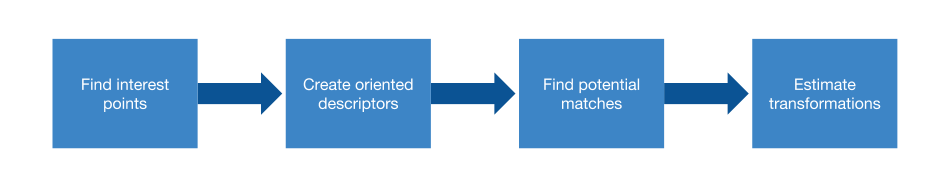
\includegraphics[width=1.0\linewidth]{./gfx/cm_pipeline.png}

\subsection*{Interest points}
To get interest points, we found the Harris corners, or points that have a high gradient in both the x and y direction within a 3x3 window [?]. We then use one of two methods to select a subset of the Harris corners: Adaptive Non-Maximal Suppression (ANMS) or gradient-based sorting. In ANMS, ... . In gradient-based sorting, we take the Harris corners that have the highest gradient, regardless of their distance to other points. 

\subsection*{Descriptors}
We experimented with two different descriptors, the box descriptor and SIFT (scale invariant feature transform).

For the box descriptor, we first implemented a naive box descriptor that did not take orientation into account. The box descriptor is created by sampling a 40 x 40 window that is Gaussian blurred (at $\sigma = 1.0$) and then downsampled to an 8 x 8 window, which is subsequently rescaled such that the features are zero mean unit variance. This descriptor worked well in identifying strictly translational copy move instances, but was a poor descriptor for rotated copy move instances.

In order to make our box descriptor rotationally invariant, we oriented the images such that the dominant gradient direction was aligend with the axis of the 40 x 40 window. The dominant gradient was found by bucketing each pixel's orientation into ten 36 degree buckets, which was weighted by the gaussian coefficient based on each pixel's distance to the central interest point and the magnitude of each pixel's gradient. The weighted average of all the point orientations that were a part of the dominant gradient direction was used to then calculate the overall weighted orientation of the descriptor.

For SIFT, for each interest point, we take a 16x16 window around that point, splitting it into 4x4 windows. For each 4x4 window, we calculate the orientation and magnitude of the gradient at that point and bucket them into 8 buckets. We do this for each of the 16 4x4 windows for a total of 128 feature descriptors. Then, we subtract the magnitude and orientation of the interest point and normalize. To avoid any values that are significantly higher than the rest, we threshold the normalized vector at 0.2 and renormalize.

\subsection*{Matching}
After we have descriptors, we use the 

Want to reduce the number of potential matches (filtering)

\subsection*{Estimated Transformations}
We use RANSAC.

\section*{Results}

We benchmark our results on two metrics: number of points that were correctly matched, and time in seconds for completion. Additionally, we evaluate our results empirically and provide some examples that worked well and others that worked less well. Our numeric metrics are displayed in Table 1. 

\begin{table}[t]
\caption{Evaluation Metrics for Image: ?}
\label{image}
\begin{center}
\begin{tabular}{l|llllll}
\multicolumn{1}{l}{} & \multicolumn{1}{l}{\bf Box, ANMS} & \multicolumn{1}{l}{\bf Box, High} & \multicolumn{1}{l}{\bf BR, ANMS} & \multicolumn{1}{l}{\bf BR, High} & \multicolumn{1}{l}{\bf SIFT, ANMS} & \multicolumn{1}{l}{\bf SIFT, High}
\\ \hline \\
{\bf \# Points} & 0 & 0 & 0 & 0 & 0 & 0 \\
{\bf Time (s)} & 0 & 0 & 0 & 0 & 0 & 0 \\
\end{tabular}
\end{center}
\end{table}

\section*{Discussion and Future Work}

Discuss here...

\subsection*{Acknowledgements}

We would like thank Alyosha Efros for teaching and inspiration, as well as the ideas from his panorama stitching project which greatly influenced our work. We would additionally like to thank the University of Nurnberg for the dataset [?].

\subsection*{References}

\begin{enumerate}
\item B. Shivakumar et al. {\it Automated Forensic Method for Copy-Move Forgery Detection based on Harris Interest Points and SIFT Descriptors}. IJCA, August 2011. 
\item {\it Image Manipulation Dataset}. http://www5.cs.fau.de/research/data/image-manipulation. 
\item J. Fridrich, D. Soukal and J. Lukas. {\it Detection of Copy-Move Forgery in Digital Images with}. Proc. of DFRWS 2003, Cleveland, OH, USA, August 5-8 2003
\item M. Brown and D. Lowe. {\it Automatic Panoramic Image Stitching using Invariant Features.} International Journal of Computer Vision. 74(1), pages 59-73, 2007.
\item M. Brown, R. Szeliski and S. Winder. {\it Multi-Image Matching using Multi-Scale Oriented Patches}. International Conference on Computer Vision and Pattern Recognition (CVPR2005) pp. 510-517.
\item S. Pittala. {\it Copy Move Forgery Detection using HOG Descriptor}.
\end{enumerate}

\end{document}

\subsection*{Appendix}

Image and stuff go here...
